\begin{frame}{Conclusion}
    \begin{itemize}
        \item \textcolor{HHturquoise_d}{\textbf{Search for non-resonant HH production and measurement of Higgs self-coupling}}
        \begin{itemize}
            \item \textbf{HH$\to b\bar{b}\gamma\gamma$} \textcolor{HHred}{\textbf{golden channel}} due to excellent signal extraction
            \item \textbf{Categorization based on optimized MV} to improve the analysis sensitivity 
            \item \textcolor{HHred}{\textbf{The world's best $\kappa_{\lambda}$ limit}}
            \item \textbf{$\times$5} improvement w.r.t previous results
            \item \textbf{Extrapolation} to Run-3 and to HL-LHC 
            \item \textbf{Interpretation in terms of EFT} can allow combining with other fields and search for BSM in a model independent way
        \end{itemize}
        \item \textcolor{HHturquoise_d}{\textbf{Photon identification using Convolutional Neural Network}}
        \begin{itemize}
            \item \textbf{New photon identification algorithm}
            \item \textcolor{HHred}{\textbf{Significance improvement}} in different events topologies
            \item Less effects from the \textbf{shower shape mis-modelling}
            \item \textbf{Possible improvements} and \textbf{baseline for Run-3 analysis}
        \end{itemize}
        \item \textcolor{HHturquoise_d}{\textbf{Parallel work}}
        \begin{itemize}
            \item \textbf{96h of lab work} at the Savoie Mont Blanc University
        \end{itemize}
    \end{itemize}
\end{frame}

{
%\usebackgroundtemplate{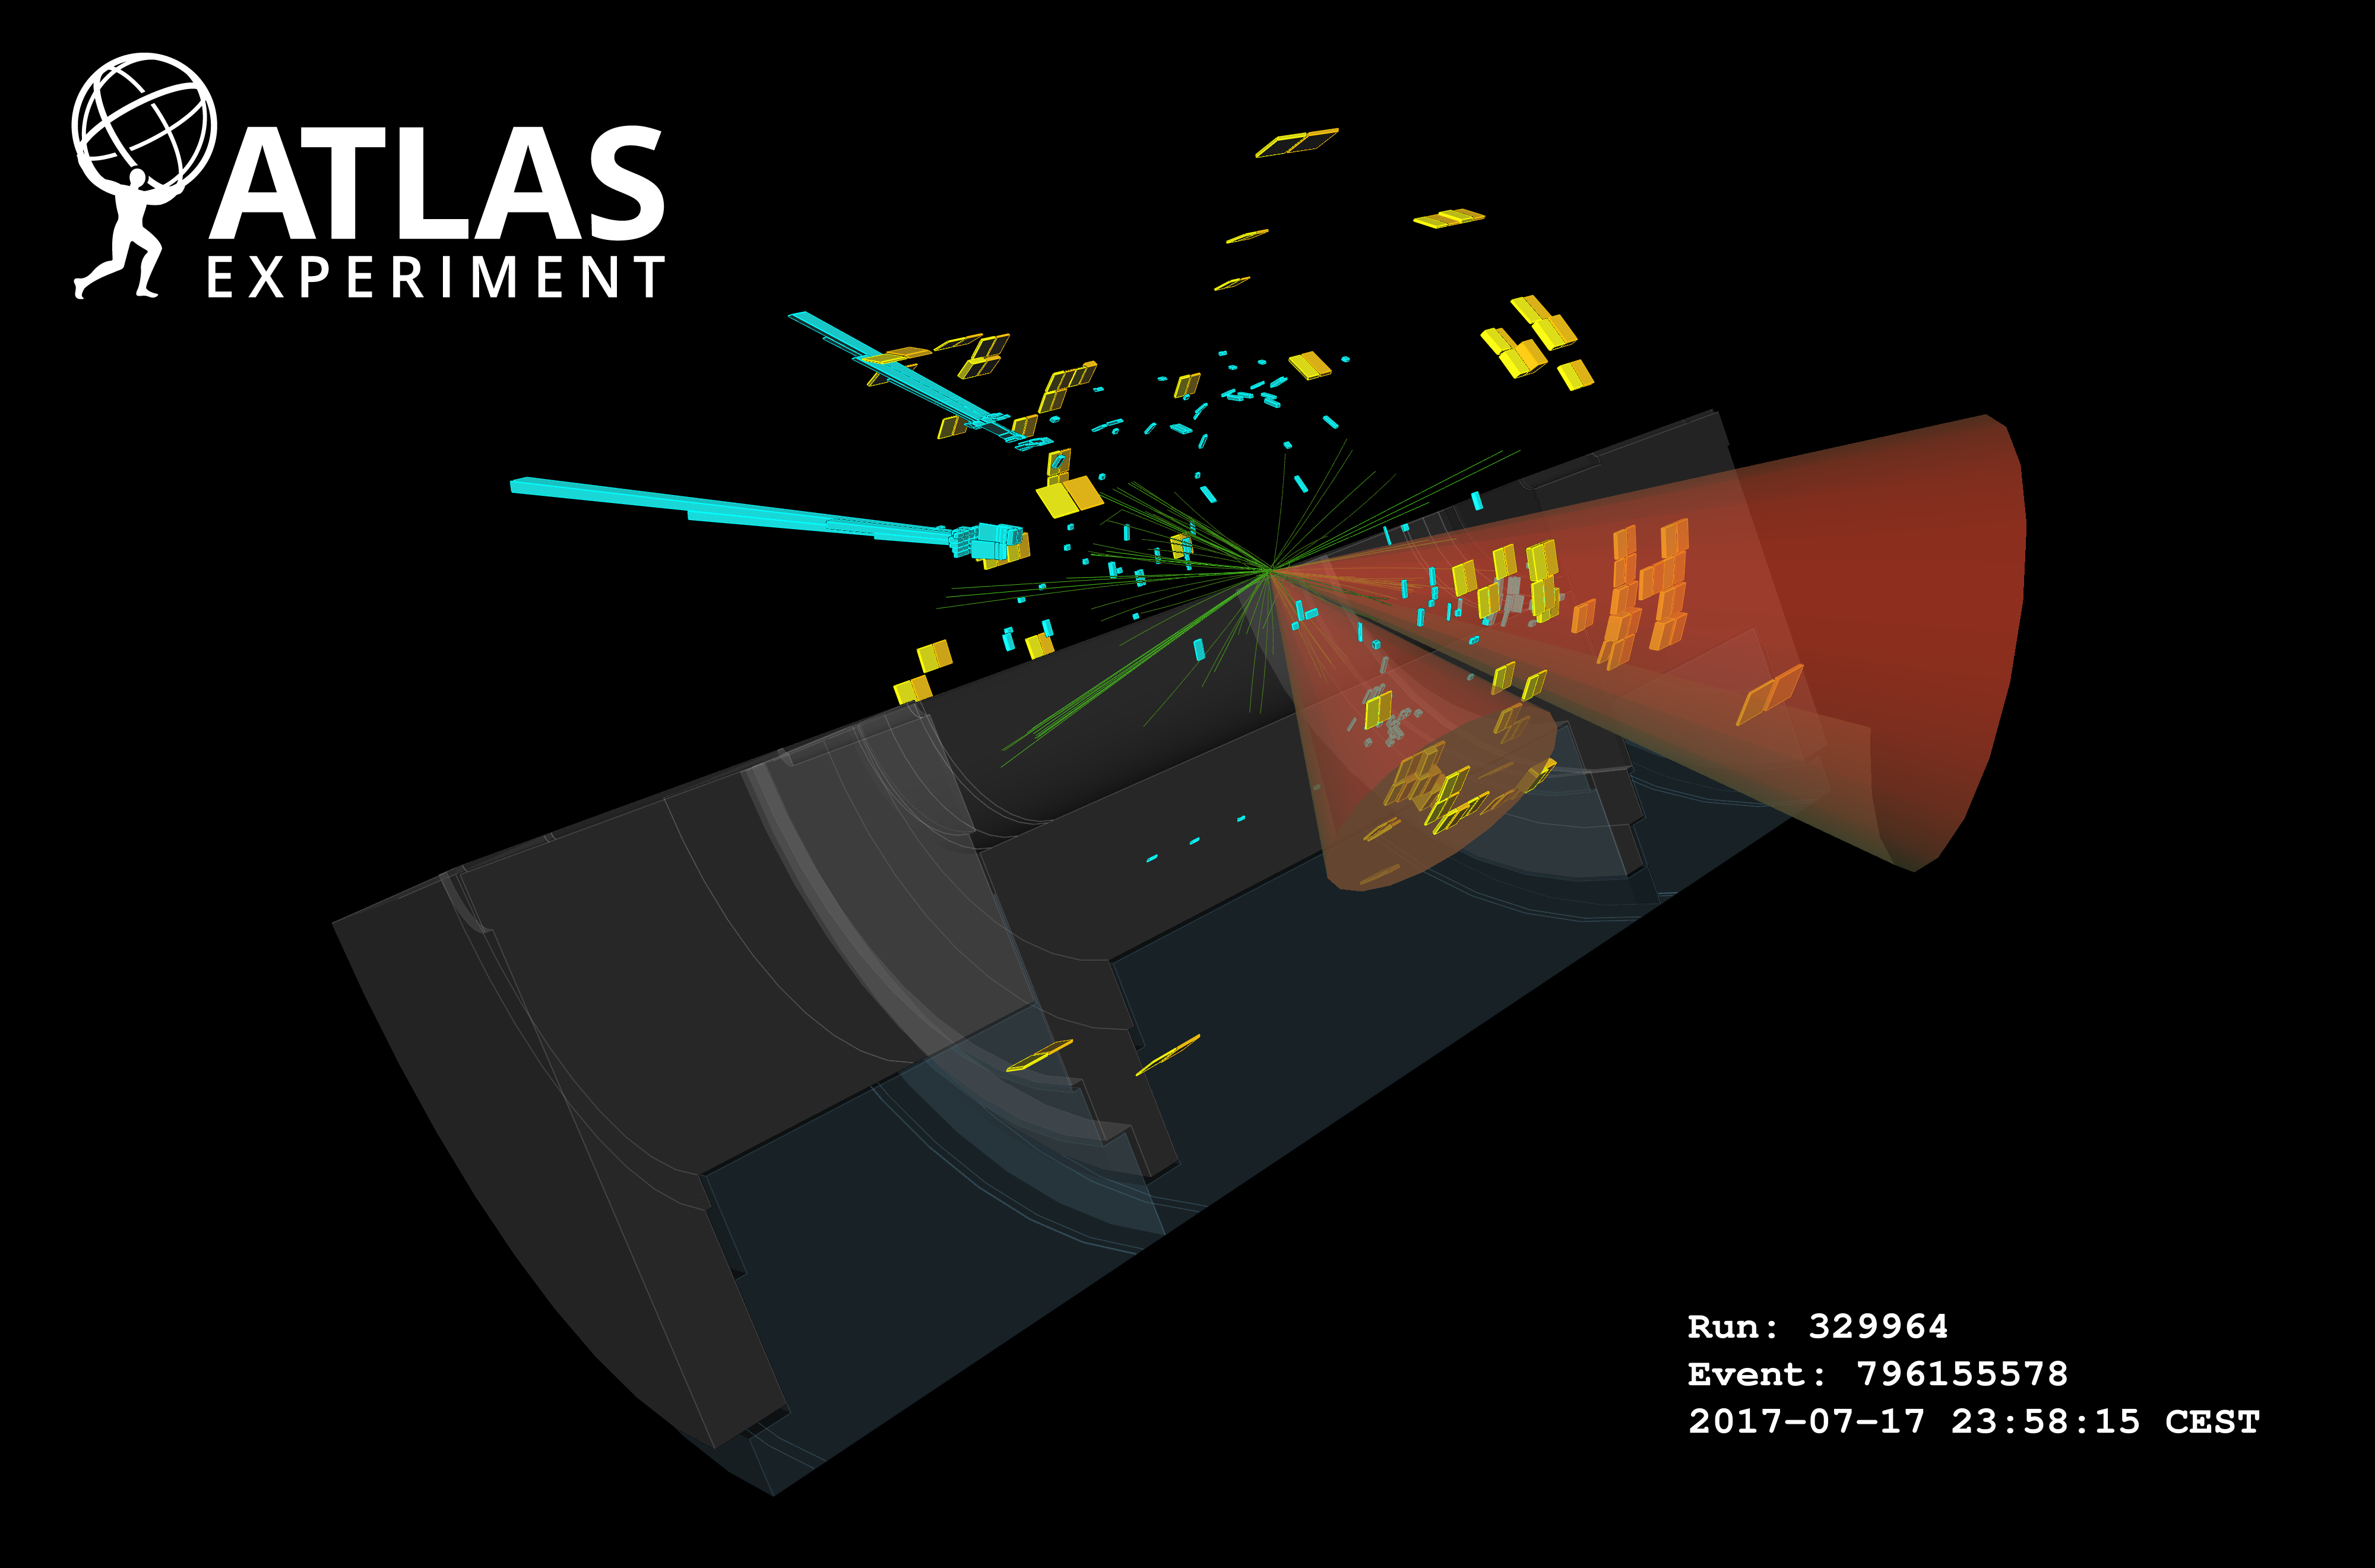
\includegraphics[width=1.2\paperwidth]{Img/figaux_01}}
\begin{frame}
\begin{center}
       \Huge\textbf{Thank you for your attention}
    \end{center}
\end{frame}
}

\begin{frame}
\begin{center}
       \Huge\textbf{BACKUP}
    \end{center}
\end{frame}

